% This file was created with tikzplotlib v0.10.1.
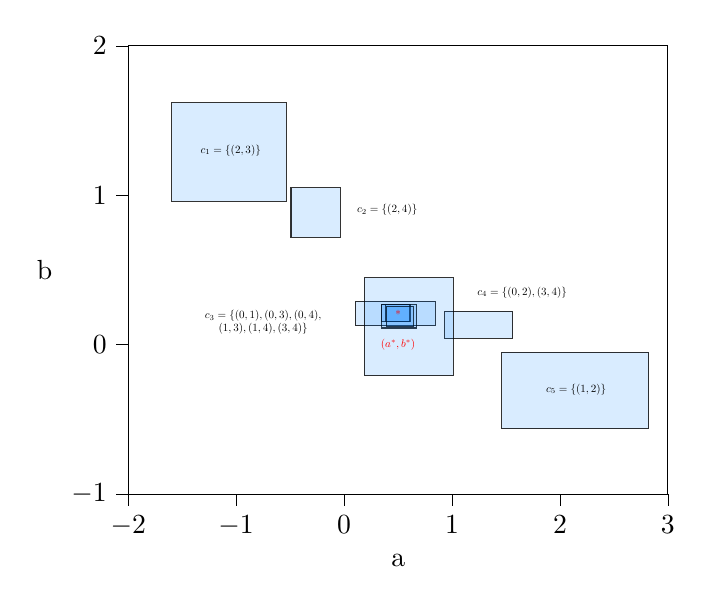
\begin{tikzpicture}

\definecolor{darkgray176}{RGB}{176,176,176}
\definecolor{dodgerblue0127255}{RGB}{0,127,255}

\begin{axis}[
tick align=outside,
tick pos=left,
x grid style={darkgray176},
xlabel={a},
xmin=-2, xmax=3,
xtick style={color=black},
y grid style={darkgray176},
ylabel style={rotate=-90.0},
ylabel={b},
ymin=-1, ymax=2,
ytick style={color=black}
]
\draw[draw=black,fill=dodgerblue0127255,draw opacity=0.8,fill opacity=0.15] (axis cs:0.103049691798598,0.126346143437506) rectangle (axis cs:0.84655997725337,0.290600627193831);
\draw[draw=black,fill=dodgerblue0127255,draw opacity=0.8,fill opacity=0.15] (axis cs:0.930837821639656,0.0433664207936635) rectangle (axis cs:1.5643006823862,0.222134384731715);
\draw[draw=black,fill=dodgerblue0127255,draw opacity=0.8,fill opacity=0.15] (axis cs:0.349241978476653,0.15339106656968) rectangle (axis cs:0.612632439528712,0.270238096995145);
\draw[draw=black,fill=dodgerblue0127255,draw opacity=0.8,fill opacity=0.15] (axis cs:0.381078919537523,0.154518861415568) rectangle (axis cs:0.602877474795857,0.267604867975125);
\draw[draw=black,fill=dodgerblue0127255,draw opacity=0.8,fill opacity=0.15] (axis cs:1.4615133317748,-0.563092838254457) rectangle (axis cs:2.82202717078302,-0.0512218400493482);
\draw[draw=black,fill=dodgerblue0127255,draw opacity=0.8,fill opacity=0.15] (axis cs:0.349919568176713,0.111483998440627) rectangle (axis cs:0.673528557342961,0.269751224992771);
\draw[draw=black,fill=dodgerblue0127255,draw opacity=0.8,fill opacity=0.15] (axis cs:0.391934576164473,0.122109089477956) rectangle (axis cs:0.639688093040606,0.25761937761001);
\draw[draw=black,fill=dodgerblue0127255,draw opacity=0.8,fill opacity=0.15] (axis cs:-1.5975153578494,0.959962938367616) rectangle (axis cs:-0.53577718318384,1.62054776942327);
\draw[draw=black,fill=dodgerblue0127255,draw opacity=0.8,fill opacity=0.15] (axis cs:-0.49136755797197,0.719574629343523) rectangle (axis cs:-0.0372395827602442,1.05076005386169);
\draw[draw=black,fill=dodgerblue0127255,draw opacity=0.8,fill opacity=0.15] (axis cs:0.186253193237637,-0.207242844407753) rectangle (axis cs:1.01376194736376,0.446813779945884);
\draw (axis cs:0.5,0.2) node[
  scale=0.4,
  text=red,
  rotate=0.0
]{*};
\draw (axis cs:0.5,0) node[
  scale=0.4,
  text=red,
  rotate=0.0
]{$(a^*,b^*)$};
\draw (axis cs:-1.05,1.3) node[
  scale=0.4,
  text=black,
  rotate=0.0
]{$c_1 = \{(2,3)\}$};
\draw (axis cs:0.4,0.9) node[
  scale=0.4,
  text=black,
  rotate=0.0
]{$c_2 = \{(2,4)\}$};
\draw (axis cs:-0.75,0.15) node[
  scale=0.4,
  text=black,
  rotate=0.0,
  align=center
]{$c_3 = \{(0, 1), (0, 3), (0, 4),$ \\$(1, 3), (1, 4), (3, 4)\}$};
\draw (axis cs:1.65,0.35) node[
  scale=0.4,
  text=black,
  rotate=0.0
]{$c_4 = \{(0,2),(3,4)\}$};
\draw (axis cs:2.15,-0.3) node[
  scale=0.4,
  text=black,
  rotate=0.0
]{$c_5 = \{(1,2)\}$};
\end{axis}

\end{tikzpicture}
